%
% A partir del fichero.pdf se genera el fichero a imprimir:
%
% pdfnup --nup 1x2 --paper a4paper --no-landscape filename.pdf
%
\documentclass[handout]{beamer}
\usepackage[latin1]{inputenc}
\usepackage[spanish]{babel}
\usepackage{amsmath,amsfonts}
\usepackage{bm}
\usepackage{epic}
\usepackage{eepic}
\newcommand{\diver}{\operatorname{{\bf div}}}
\mode<presentation>
{
  \usetheme{PaloAlto}
  % or ...

%  \setbeamercovered{transparent}
  % or whatever (possibly just delete it)
  \usecolortheme{dove}
}

\title[Tecnología de elementos]{MÉTODO DE LOS ELEMENTOS FINITOS \\
Tecnología de elementos}
\author[F. Gabaldón]{Felipe Gabaldón Castillo}
\date{}
\pgfdeclareimage[height=0.5cm]{logo-upm}{upm}
\logo{\pgfuseimage{logo-upm}}

\AtBeginSection[]
{
  \begin{frame}<beamer>
    \frametitle{Índice}
    \tableofcontents[currentsection]
  \end{frame}
}
%%%%%%%%%%%%%%%%%%%%%%%%%%%%%%%%%%%%%%%%%%%%%%%%%%%%%%%%%%%%%%%%%%%%%%%%%%%%%%
\newcommand{\norm}[1]{\lVert #1 \rVert}
\begin{document}
%%%%%%%%%%%%%%%%%%%%%%%%%%%%%%%%%%%%%%%%%%%%%%%%%%%%%%%%%%%%%%%%%%%%%%%%%%%%%%
\begin{frame}
\titlepage
\end{frame}
%%%%%%%%%%%%%%%%%%%%%%%%%%%%%%%%%%%%%%%%%%%%%%%%%%%%%%%%%%%%%%%%%%%%%%%%%%%%%%
\begin{frame}
\frametitle{Índice}
\tableofcontents
\end{frame}
%%%%%%%%%%%%%%%%%%%%%%%%%%%%%%%%%%%%%%%%%%%%%%%%%%%%%%%%%%%%%%%%%%%%%%%%%%%%%%
\section{El fenómeno de bloqueo}
%%%%%%%%%%%%%%%%%%%%%%%%%%%%%%%%%%%%%%%%%%%%%%%%%%%%%%%%%%%%%%%%%%%%%%%%%%%%%%
\begin{frame}
\frametitle{Introducción}
\begin{itemize}
\item Ciertas restricciones físicas conducen a situaciones de bloqueo de
la formulación en desplazamientos. Ejemplos:
\begin{itemize}
\item Elasticidad incompresible ($\nu \rightarrow 0.5$).
\item Flexión de vigas y placas delgadas ($t \rightarrow 0.5$).
\end{itemize}
\item {\bf Concepto:} La
metodología de solución es minimizar la energía
potencial total. Utilizar para ello el método de los elementos finitos
ya introduce una restricción (se busca el mínimo para una cierta clase de
desplazamientos, por ejemplo polinomios continuos a trozos). Si además existen
restricciones adicionales de tipo físico, el sistema puede quedar con un
exceso de restricciones que hagan que la única solución del sistema sea
la nula.
\item Pueden existir restricciones ``escondidas'':
plasticidad con deformaciones plásticas de carácter isocórico.
\item El problema debe plantearse introduciendo una incógnita por cada ecuación
de restricción.
\end{itemize}
\end{frame}
%%%%%%%%%%%%%%%%%%%%%%%%%%%%%%%%%%%%%%%%%%%%%%%%%%%%%%%%%%%%%%%%%%%%%%%%%%%%%%
\begin{frame}
\frametitle{Elasticidad incompresible}
\begin{itemize}
\item Ecuación constitutiva (medio elástico isótropo):
$$
\sigma_{ij}=\lambda u_{k,k} \delta_{ij}+2 \mu u_{(i,j)}
$$

Si $\nu \rightarrow \frac{1}{2}$, entonces $\lambda=\frac{2 \nu \mu}{1-2\nu}
\rightarrow \infty$

La formulación en este caso será:
\begin{align*}
\sigma_{ij}&=-p \delta_{ij}+2 \mu u_{(i,j)} \\
u_{i,i}&=0
\end{align*}
\item Para triángulos lineales de presión constante, se tiene:
$$\int_{\Omega_e} \delta p^h u^h_{i,i} d\Omega=0 \;\; \forall \delta p^h \mbox{cte en
} \Omega_e
\Rightarrow \int_{\Omega_e} u^h_{i,i} d\Omega=0$$
es decir, los elementos no cambian de volumen:
\end{itemize}
\end{frame}
%%%%%%%%%%%%%%%%%%%%%%%%%%%%%%%%%%%%%%%%%%%%%%%%%%%%%%%%%%%%%%%%%%%%%%%%%%%%%%
\begin{frame}
\frametitle{Elasticidad incompresible}
\begin{center}
\includegraphics[width=0.9\textwidth]{bloqueo.pdf}
\end{center}
\end{frame}
%%%%%%%%%%%%%%%%%%%%%%%%%%%%%%%%%%%%%%%%%%%%%%%%%%%%%%%%%%%%%%%%%%%%%%%%%%%%%%
\begin{frame}
\frametitle{El fenómeno del bloqueo. Elasticidad incompresible}
\begin{itemize}
\item Formulación válida para medios compresibles e incompresibles:
\begin{align*}
\sigma_{ij}&=-p \delta_{ij}+2 \mu u_{(i,j)} \\
u_{i,i}+\frac{p}{\lambda}&=0
\end{align*}
\item Observaciones
\begin{align*}
\nu&=\frac{1}{2} \Rightarrow p=-\frac{\sigma_{ii}}{3} \\
\nu &\approx \frac{1}{2} \Rightarrow p \approx -\frac{\sigma_{ii}}{3} \\
\nu &\neq \frac{1}{2} \Rightarrow p=-\lambda u_{i,i} \neq
\frac{\sigma_{ii}}{3}
\end{align*}
\end{itemize}
\end{frame}
%%%%%%%%%%%%%%%%%%%%%%%%%%%%%%%%%%%%%%%%%%%%%%%%%%%%%%%%%%%%%%%%%%%%%%%%%%
\section{La prueba de la parcela}
%%%%%%%%%%%%%%%%%%%%%%%%%%%%%%%%%%%%%%%%%%%%%%%%%%%%%%%%%%%%%%%%%%%%%%%%%%
\begin{frame}
\frametitle{La prueba de la parcela}
\begin{small}
\begin{itemize}
\item Introducida originalmente por Irons en 1965 y revisada posteriormente
por Taylor et al. en 1986 (Individual patch test). 
\item Los estados de deformación constante (incluyendo movimientos
de sólido rígido) han de ser representados de manera exacta.
\item Ha de verificarse, en particular, para un solo elemento.
\item Se debe probar sobre elementos distorsionados.
%\item En teoría solo necesita cumplirse en el límite en que $h \rightarrow 0$
%\item Sirve como chequeo de que no existen modos espúreos de energía nula, 
%garantizando la estabilidad numérica de la formulación.
\item Los modos de deformación constante y de sólido rígido son
capturados de manera exacta por todos los elementos que pasan la
prueba de la parcela. La diferencia entre los distintos elementos se
encuentra en la rigidez de los modos de flexión.
\item Los modos de flexión no han de tener rigidez infinita en el
límite incompresible. Este es el problema que tiene la formulación en
desplazamientos.
\item Asimismo, dichos modos no han de tener rigidez nula.
La formulación con integración reducida da lugar
a modos espúreos de flexión con energía nula $\rightarrow$ hourglassing.
\end{itemize}
\end{small}
\end{frame}
%%%%%%%%%%%%%%%%%%%%%%%%%%%%%%%%%%%%%%%%%%%%%%%%%%%%%%%%%%%%%%%%%%%%%%%%%%
\section{Análisis espectral (Q4)}
%%%%%%%%%%%%%%%%%%%%%%%%%%%%%%%%%%%%%%%%%%%%%%%%%%%%%%%%%%%%%%%%%%%%%%%%%%
\begin{frame}
\frametitle{Modos de deformación}
\begin{itemize}
\item Para el elemento bilineal de $4$ nodos los modos de deformación son:

\vspace{5mm}
\includegraphics{modosq4}
\end{itemize}
\end{frame}
%%%%%%%%%%%%%%%%%%%%%%%%%%%%%%%%%%%%%%%%%%%%%%%%%%%%%%%%%%%%%%%%%%%%%%%%%%
\begin{frame}
\frametitle{Autovalores}
\begin{itemize}
\item Modos de sólido rígido
\begin{equation*}
\lambda_{\textrm{SR1}}=0, \quad
\lambda_{\textrm{SR2}}=0, \quad
\lambda_{\textrm{SR3}}=0
\end{equation*}
\item Modo volumétrico
\begin{multline*}
\lambda_{\textrm{VOL}}=\frac{1}{2r}\left[
(\lambda+2\mu)(1+r^2)+ \right.\\
\left. \sqrt{4 \mu (\lambda+\mu)(r^2-1)^2+\lambda^2(r^2+1)^2}
\right] \qquad r=\frac{h}{b}
\end{multline*}
En el caso incompresible $\lambda_{\textrm{VOL}}\rightarrow \infty$
\item Flexión
\begin{equation*}
\lambda_{\textrm{BG1}}=\frac{\mu+(\lambda+2\mu)r^2}{3r}, \quad
\lambda_{\textrm{BG2}}=\frac{\mu r^2+\lambda+2\mu}{3r}
\end{equation*}
con $r=h/b$.
En el problema de flexión de vigas delgadas $\lambda_{\textrm{BG1}} 
\rightarrow \infty$ ó $\lambda_{\textrm{BG2}} \rightarrow \infty$ 
\end{itemize}
\end{frame}
%%%%%%%%%%%%%%%%%%%%%%%%%%%%%%%%%%%%%%%%%%%%%%%%%%%%%%%%%%%%%%%%%%%%%%%%%%
\begin{frame}
\frametitle{Conclusiones}
\begin{itemize}
\item El fenómeno del bloqueo aparece como consecuencia de una formulación
numérica inadecuada que da lugar a un problema con demasiadas restricciones.
En concreto, dos defectos clave son la interpolación lineal de las respuestas
volumétricas y de corte.
\item El problema debe solucionarse modificando la 
formulación en los términos que dan lugar a los campos de deformaciones no
constantes. La integración reducida elimina la parte no constante de las
deformaciones en el elemento, pero da lugar a modos espúreos de energía
nula.
\end{itemize}
\end{frame}
%%%%%%%%%%%%%%%%%%%%%%%%%%%%%%%%%%%%%%%%%%%%%%%%%%%%%%%%%%%%%%%%%%%%%%%%%%
\begin{frame}
\frametitle{Tecnologías especiales}
\begin{enumerate}
\item Métodos mixtos.
\item Integración selectiva y reducida.
\item Control de Hourglass
\item Formulación $\overline{\bm{B}}$
\item El método de los modos incompatibles
\item Formulación con deformaciones supuestas mejoradas
\end{enumerate}
\end{frame}
%%%%%%%%%%%%%%%%%%%%%%%%%%%%%%%%%%%%%%%%%%%%%%%%%%%%%%%%%%%%%%%%%%%%%%%%%%
\section{Formulaciones mixtas}
%%%%%%%%%%%%%%%%%%%%%%%%%%%%%%%%%%%%%%%%%%%%%%%%%%%%%%%%%%%%%%%%%%%%%%%%%%
\begin{frame}
\frametitle{Introducción}
\begin{itemize}
\item Las referencias son muy abundantes
\item Los métodos mixtos emplean diferentes interpolaciones para diferentes
campos: desplazamientos-presión, desplazamientos-tensión,
desplazamientos-deformación, etc.
\item Para que una formulación mixta tenga garantizada la convergencia, ha de
verificar la condición de Babuska-Brezzi (problema de checker-board).
\item Los elementos de orden alto pierden robustez en problemas no lineales.
\item No hay un ``buen elemento'' para todas las clases de problemas
\end{itemize}
\end{frame}
%%%%%%%%%%%%%%%%%%%%%%%%%%%%%%%%%%%%%%%%%%%%%%%%%%%%%%%%%%%%%%%%%%%%%%%%%%
\begin{frame}
\frametitle{Formulación fuerte}
\begin{itemize}
\item Dados $\bm{f}$, $\bm{g}$, $\bm{h}$,
encontrar $\bm{u}:\Omega \rightarrow R$, $p:\Omega \rightarrow R$
tal que:
\begin{align*}
\sigma_{ij,j}+f_{i}&=0 \;\;\;\; \mbox{en } \Omega\\
u_{i,i}+p/\lambda&=0 \;\;\;\; \mbox{en } \Omega\\
u_{i}&=\overline{u}_{i} \;\;\;\; \mbox{en } \partial_{u}\Omega\\
\sigma_{ij} n_{j}&=\overline{t}_i  \;\;\;\; \mbox{en } \partial_{t}\Omega
\end{align*}
siendo:
$$\sigma_{ij}=-p \delta_{ij} + 2\mu u_{(i,j)}$$
\end{itemize}
\end{frame}
%%%%%%%%%%%%%%%%%%%%%%%%%%%%%%%%%%%%%%%%%%%%%%%%%%%%%%%%%%%%%%%%%%%%%%%%%%
\begin{frame}
\frametitle{Formulación débil}
\begin{itemize}
\item Sean:
\begin{align*}
{\cal U}&=\mbox{espacio de las soluciones de prueba (desplazamientos)} \\
{\cal V}&=\mbox{espacio de las funciones de peso (desplazamientos)} \\
{\cal P}&=\mbox{espacio de las presiones}
\end{align*}
Dados $f_{i}$, $\overline{u}_{i}$, $\overline{t}_{i}$,
encontrar $u_{i} \in {\cal U}$ y $p\in {\cal P}$
tal que $\forall \delta u_{i} \in {\cal V}$, $\delta p \in {\cal P}$, se
verifique:
\begin{multline}
\int_{\Omega} \delta u_{(i,j)} \sigma_{ij} d\Omega-\int_{\Omega}
\delta p \left(
u_{i,i}+\frac{p}{\lambda} \right) d\Omega
=\int_{\Omega} \delta u_{i} f_{i} d\Omega + \\
\int_{\partial_{t}\Omega}
\delta u_{i} \overline{t}_{i} d \Gamma \label{fdebinco}
\end{multline}
\end{itemize}
\end{frame}
\newpage
%%%%%%%%%%%%%%%%%%%%%%%%%%%%%%%%%%%%%%%%%%%%%%%%%%%%%%%%%%%%%%%%%%%%%%%%%%
\begin{frame}
\frametitle{Método de Galerkin}
\begin{itemize}
\item Sean:
\begin{align*}
S_{i}^{h}&=\mbox{espacio de las soluciones de prueba (desplazamientos)} \\
\nu_{i}^{h}&=\mbox{espacio de las funciones de peso (desplazamientos)} \\
{\cal P}^h&=\mbox{aproximación del espacio de las presiones}
\end{align*}
Dados $f_{i}$, $\overline{u}_{i}$, $\overline{t}_{i}$,
encontrar $u_{i}^{h} \in S_{i}^{h}$ y $p\in {\cal P}^{h}$
tal que $\forall \delta u_{i}^{h}\in \nu_{i}^{h}$, $\delta p^{h}
\in {\cal P}^{h}$, se verifique:
\begin{multline}
\int_{\Omega} \delta u_{(i,j)}^{h} \sigma_{ij}^{h} d\Omega-
\int_{\Omega} \delta p^{h} \left(
u_{i,i}^{h}+\frac{p^{h}}{\lambda} \right) d\Omega
=\int_{\Omega} \delta u_{i}^{h} f_{i} d\Omega + \\
\int_{\partial_{t}\Omega}
\delta u_{i}^{h} \overline{t}_{i} d \Gamma \label{metgainco}
\end{multline}
\end{itemize}
\end{frame}
%%%%%%%%%%%%%%%%%%%%%%%%%%%%%%%%%%%%%%%%%%%%%%%%%%%%%%%%%%%%%%%%%%%%%%%%%%
\begin{frame}
\frametitle{Interpolación del campo de presiones}
\begin{itemize}
\item La interpolación de desplazamientos es la estándar. La de presiones 
puede ser discontinua
\item ¡ No todos los elementos funcionan !:
\end{itemize}
$$r=\frac{n_{eq}}{n_{c}}; \qquad
\begin{array}{lll}
n_{eq}&\equiv &\textrm{ ecuaciones en desplazamientos} \\
n_{c} &\equiv &\textrm{ restricciones de incompresibilidad}
\end{array}
$$
\begin{align*}
r&=2 \;\;\;\;\;\mbox{óptimo} \\
r&>2 \;\;\;\;\;\mbox{pocas restricciones de incompresibilidad} \\ 
r&<2 \;\;\;\;\;\mbox{demasiadas restricciones de incompresibilidad} \\
r&\leq1 \;\;\;\;\;\mbox{bloqueo severo}
\end{align*}
\end{frame}
%%%%%%%%%%%%%%%%%%%%%%%%%%%%%%%%%%%%%%%%%%%%%%%%%%%%%%%%%%%%%%%%%%%%%%%%%%
\begin{frame}
\frametitle{Interpolación del campo de presiones}

\begin{center}
\includegraphics{dis-p-el}
\end{center}
\end{frame}
%%%%%%%%%%%%%%%%%%%%%%%%%%%%%%%%%%%%%%%%%%%%%%%%%%%%%%%%%%%%%%%%%%%%%%%%%%
\section{Integración selectiva}
%%%%%%%%%%%%%%%%%%%%%%%%%%%%%%%%%%%%%%%%%%%%%%%%%%%%%%%%%%%%%%%%%%%%%%%%%%
\begin{frame}
\frametitle{Integración selectiva y reducida}
\begin{itemize}
\item Concepto:

\begin{align*}
\bm{K}^{e}&=\int_{\Omega_{e}} \bm{B}^{\rm T} \bm{D} \bm{B} d \Omega \\
\mbox{}   &=
\underbrace{\int_{\Omega_{e}} \bm{B}^{\rm T} \bm{D}_{\lambda} \bm{B} d \Omega}_{\mbox{Int. red: } 1\times 1}
+
\underbrace{\int_{\Omega_{e}} \bm{B}^{\rm T} \bm{D}_{\mu} \bm{B} d \Omega}_{\mbox{Int. comp: } 2\times 2}
\end{align*}
siendo:
$$\sigma_{ij}=\lambda \epsilon_{kk} \delta_{ij}+
2 \mu \epsilon_{ij}$$

\item Formulación en desplazamientos.

\item Teorema de equivalencia (Malkus-Hughes)
\end{itemize}
\end{frame}
%%%%%%%%%%%%%%%%%%%%%%%%%%%%%%%%%%%%%%%%%%%%%%%%%%%%%%%%%%%%%%%%%%%%%%%%%%
\section{Control de Hourglass}
%%%%%%%%%%%%%%%%%%%%%%%%%%%%%%%%%%%%%%%%%%%%%%%%%%%%%%%%%%%%%%%%%%%%%%%%%%
\begin{frame}
\frametitle{Control de ``hourglass''}
\begin{itemize}
\item Concepto: utilizar integración reducida añadiendo rigidez artificial a
los modos de flexión.
\item Utiliza parámetros escogidos 
``ad-hoc'' para introducir la rigidez artificial.
%\item Es muy popular en los programas explícitos.
\end{itemize}
\end{frame}
%%%%%%%%%%%%%%%%%%%%%%%%%%%%%%%%%%%%%%%%%%%%%%%%%%%%%%%%%%%%%%%%%%%%%%%%%%
\section{Formulacion B-bar}
%%%%%%%%%%%%%%%%%%%%%%%%%%%%%%%%%%%%%%%%%%%%%%%%%%%%%%%%%%%%%%%%%%%%%%%%%%
\begin{frame}
\frametitle{La formulación $\overline{\bm{B}}$}
\begin{itemize}
\item Concepto: $\bm{\varepsilon}=\overline{\bm{B}} \bm{d}$
\item Ejemplo: elemento de $4$ nodos bidimensional
$$\bm{B}=(\bm{B}^{1},\bm{B}^2,\bm{B}^3,\bm{B}^4); \qquad
\bm{B}^{A}=\left(
\begin{array}{cc}
N^{A}_{,1}&0\\
0&N^{A}_{,2}\\
N^{A}_{,2}&N^{A}_{,1}
\end{array}
\right)
$$
Se considera la descomposición aditiva de $\bm{B}$ en:
$\bm{B}=\bm{B}_{\rm vol}+\bm{B}_{\rm dev}$,
siendo:
$$\bm{B}^{A}_{\rm vol}=\frac{1}{3}
\left(
\begin{array}{cc}
N^{A}_{,1}&N^{A}_{,2}\\
N^{A}_{,1}&N^{A}_{,2}\\
0&0
\end{array}
\right)
\;\;\mbox{y }\;\; \bm{B}_{\rm dev}=\bm{B}-\bm{B}_{dev}$$
Se define:
$\overline{\bm{B}}=\left. \bm{B}_{\rm vol}\right|_{\bm{\xi}=\bm{0}}+\bm{B}_{\rm dev}$
\end{itemize}
\end{frame}
%%%%%%%%%%%%%%%%%%%%%%%%%%%%%%%%%%%%%%%%%%%%%%%%%%%%%%%%%%%%%%%%%%%%%%%%%%
\section{Modos incompatibles}
%%%%%%%%%%%%%%%%%%%%%%%%%%%%%%%%%%%%%%%%%%%%%%%%%%%%%%%%%%%%%%%%%%%%%%%%%%
\begin{frame}
\frametitle{El método de los modos incompatibles}
\begin{itemize}
\item Concepto: añadir modos de flexión de orden cuadrático.
\item Interpolación del campo de desplazamientos:
$$\bm{u}=\sum_{A=1}^{4} N_{A}(\bm{\xi}) \bm{d}_{A}+\sum_{I=1}^{2}
\tilde{N}_{I}(\bm{\xi}) \bm{\alpha}_{I}$$
\begin{xalignat*}{3}
\textrm{siendo:} & \mbox{} &
\tilde{N}_{1}(\bm{\xi})&=\frac{1}{2}(\xi^2-1), &
\tilde{N}_{2}(\bm{\xi})&=\frac{1}{2}(\eta^2-1)
\end{xalignat*}
\item Los $\bm{\alpha}_{I}$ son grados de libertad internos a nivel de cada
elemento.
\item Deformaciones: $\bm{\varepsilon}=\bm{B} \bm{d} + \bm{G} \bm{\alpha}$
$$
\bm{G}=\left[ \bm{G}_{1} \; \bm{G}_{2} \right] 
\;\;\;\;\;\;
\bm{G}_{I}=
\left(
\begin{array}{cc}
\tilde{N}_{I,1}&0 \\
0& \tilde{N}_{I,2}\\
\tilde{N}_{I,2}&\tilde{N}_{I,1}
\end{array}
\right)
$$
\end{itemize}
\end{frame}
%%%%%%%%%%%%%%%%%%%%%%%%%%%%%%%%%%%%%%%%%%%%%%%%%%%%%%%%%%%%%%%%%%%%%%%%%%
\section{Deformaciones supuestas}
%%%%%%%%%%%%%%%%%%%%%%%%%%%%%%%%%%%%%%%%%%%%%%%%%%%%%%%%%%%%%%%%%%%%%%%%%%%%%%
\begin{frame}
\frametitle{Formulación E.A.S.}
\begin{itemize}
\item Del acrónimo inglés {\em Enhanced Assumed Strain}
\item Objetivo: desarrollar un 
elemento de prestaciones similares al de
Wilson-Taylor y que además tenga las características:
\begin{enumerate}
\item Formulación variacionalmente consistente
\item Formulación sistemática de diversas familias de elementos
\item Generalización para problemas con grandes deformaciones
\end{enumerate}
\item Concepto: el campo de deformaciones compatibles se mejora 
añadiendole un campo de deformaciones ``mejoradas'':
$$\bm{\varepsilon}=\bm{\nabla}^{\rm S}\bm{u}+\tilde{\bm{\varepsilon}}$$
\end{itemize}
\end{frame}
%%%%%%%%%%%%%%%%%%%%%%%%%%%%%%%%%%%%%%%%%%%%%%%%%%%%%%%%%%%%%%%%%%%%%%%%%%
\begin{frame}
\frametitle{Diseño de elementos: Metodología}
\begin{enumerate}
\item Definir en el espacio isoparamétrico una matriz de interpolación 
${\bf E}({\bm \xi})$, tal que el campo de deformaciones mejoradas tenga 
la expresión:
$$
{\tilde {\bf E}}({\bm \xi})={\bf E}({\bm \xi})\cdot {\bm \alpha}^{e}
\qquad {\bm \alpha}^{e} \in {\cal R}^{n_{\varepsilon}}
$$
\item Obtener la expresión de la matriz ${\bf G}({\bm \xi})$ de interpolación
del campo de deformaciones mejoradas en el espacio físico
${\tilde {\bm \varepsilon}}({\bm \xi})$
$$
{\bf G}({\bm \xi})=\frac{j_{0}}{j({\bm \xi})}{\bf F}_{0}^{-{\rm T}}
{\bf E}({\bf \xi}) 
$$
\end{enumerate}
\end{frame}
%%%%%%%%%%%%%%%%%%%%%%%%%%%%%%%%%%%%%%%%%%%%%%%%%%%%%%%%%%%%%%%%%%%%%%%%%%
\begin{frame}
\frametitle{Diseño de elementos: Ejemplos}
\begin{footnotesize}
\begin{itemize}
\item Elemento Q4/E4 (Wilson-Taylor)
$$
{\bm E}({\bm \xi})=
\left(
\begin{array}{cccc}
\xi&0&0&0 \\
0  &\eta&0&0\\
0  &   0&\xi&\eta
\end{array}
\right)
$$
\item Elemento Q4/E5 (Simo-Rifai)
$$
{\bm E}({\bm \xi})=
\left(
\begin{array}{ccccc}
\xi&0&0&0&\xi \eta \\
0  &\eta&0&0&-\xi \eta \\
0  &   0&\xi&\eta&\xi^2-\eta^2
\end{array}
\right)
$$
\item Elemento Q4/E7 (Andelfinger-Ramm)
$$
{\bm E}({\bm \xi})=
\left(
\begin{array}{ccccccc}
\xi&0&0&0&\xi \eta&0&0 \\
0  &\eta&0&0&0&\xi \eta&0\\
0  &   0&\xi&\eta&0&0&\xi \eta
\end{array}
\right)
$$
\end{itemize}
\end{footnotesize}
\end{frame}
%%%%%%%%%%%%%%%%%%%%%%%%%%%%%%%%%%%%%%%%%%%%%%%%%%%%%%%%%%%%%%%%%%%%%%%%%%
\section{Conclusiones}
%%%%%%%%%%%%%%%%%%%%%%%%%%%%%%%%%%%%%%%%%%%%%%%%%%%%%%%%%%%%%%%%%%%%%%%%%%%%%%
\begin{frame}
\frametitle{Conclusiones}
Autovalores $(r=h/b)$. Modos de flexión
\begin{center}
\begin{small}
\begin{tabular}{||c|c|c||}
\hline \hline
& BG1 & BG2 \\ \hline \hline
$Q4$             &$(\mu+(\lambda+2\mu)r^2)/3r$&
$(\mu r^2+\lambda+2\mu)/3r$      \\
\hline
$Q4R$            &$0$
&
$0$
\\ \hline
$Q4RS$
&$\mu(2r^2+1)/3r$
&
$\mu(r^2+2)/3r$
\\
\hline
$\overline{\bm{B}}$&$(9\mu+r^2(\lambda+10\mu))/27r$
&
$(9r^2\mu+(\lambda+10\mu))/27r$
\\
\hline
$Q1/E4$
&$4r\mu(\lambda+\mu)/3(\lambda+2\mu)$
&
$4\mu(\lambda+\mu)/3r(\lambda+2\mu)$\\
\hline
\end{tabular}
\end{small}
\end{center}
\begin{itemize}
\item Elemento $Q4R$: modos de energía nula
\item Régimen incompresible $(\lambda\rightarrow\infty)$ y flexión de vigas
delgadas $(r\rightarrow\infty)$: bloqueo de
$Q4;\;Q4R;\;Q4RS;\; \overline{\bm{B}}$
\item $Q1/E4$; $Q1/E5$ y $Q1/E7$ equivalentes en paralelogramos
\end{itemize}
\end{frame}
%%%%%%%%%%%%%%%%%%%%%%%%%%%%%%%%%%%%%%%%%%%%%%%%%%%%%%%%%%%%%%%%%%%%%%%%%%%%%%
\begin{frame}
\frametitle{Ejemplos. Sensibilidad a la distorsión}

\begin{center}
\includegraphics{mens-sim}

\includegraphics{mens-asim}
\end{center}
\end{frame}
%%%%%%%%%%%%%%%%%%%%%%%%%%%%%%%%%%%%%%%%%%%%%%%%%%%%%%%%%%%%%%%%%%%%%%%%%%%%%%
\begin{frame}
\frametitle{Ejemplos. Sensibilidad a la distorsión}
\begin{small}
\begin{center}
\begin{tabular}{||c|c|c|c||}
\hline \hline
$\theta    $& $Q4$        &$\overline{B}$& $Q1/E4$   \\ \hline \hline
$0^{\circ} $&$0.12458$    &$0.12995$     &$0.99664$  \\ \hline
$15^{\circ}$&$0.11080$    &$0.11935$     &$0.96783$  \\ \hline
$30^{\circ}$&$0.08022$    &$0.09275$     &$0.91632$  \\ \hline
$45^{\circ}$&$0.04985$    &$0.06101$     &$0.88451$  \\ \hline
\end{tabular}
\end{center}

\begin{center}
\begin{tabular}{||c|c|c|c|c|c||}
\hline \hline
$\theta$& $Q4$       &$\overline{B}$&$Q1/E4$ &$Q1/E5$
&$Q1/E7$ \\ \hline \hline
$ 0^{\circ}$ & $0.12458$  &$0.12995$
&$0.99664$&$0.99664$&$0.99664$ \\ \hline
$15^{\circ}$ & $0.09959$  &$0.10467$
&$0.45105$&$0.45107$&$0.45107$ \\ \hline
$30^{\circ}$ & $0.06148$  &$0.06563$
&$0.26135$&$0.26143$&$0.26145$ \\ \hline
$45^{\circ}$ & $0.03627$  &$0.03906$
&$0.19824$&$0.19845$&$0.19849$ \\ \hline
\end{tabular}
\end{center}
\end{small}
\end{frame}
%%%%%%%%%%%%%%%%%%%%%%%%%%%%%%%%%%%%%%%%%%%%%%%%%%%%%%%%%%%%%%%%%%%%%%%%%%%%%%
\begin{frame}
\frametitle{Ejemplos. Ensayo de identación de Prandtl}
\begin{center}
\includegraphics[width=\textwidth]{punch}
\end{center}
\end{frame}
\newpage
%%%%%%%%%%%%%%%%%%%%%%%%%%%%%%%%%%%%%%%%%%%%%%%%%%%%%%%%%%%%%%%%%%%%%%%%%%%%%%
\begin{frame}
\frametitle{Ejemplos. Ensayo de identación de Prandtl}
\begin{center}
\includegraphics[width=\textwidth]{punchfd}
\end{center}
\end{frame}
%%%%%%%%%%%%%%%%%%%%%%%%%%%%%%%%%%%%%%%%%%%%%%%%%%%%%%%%%%%%%%%%%%%%%%%%%%%%%%
\begin{frame}
\frametitle{Ejemplos. La membrana de Cook}

\vspace{1cm}
\begin{center}
\includegraphics[width=0.65\textwidth]{cook}
\end{center}
\end{frame}
%%%%%%%%%%%%%%%%%%%%%%%%%%%%%%%%%%%%%%%%%%%%%%%%%%%%%%%%%%%%%%%%%%%%%%%%%%%%%%
\begin{frame}
\frametitle{Ejemplos. La membrana de Cook}

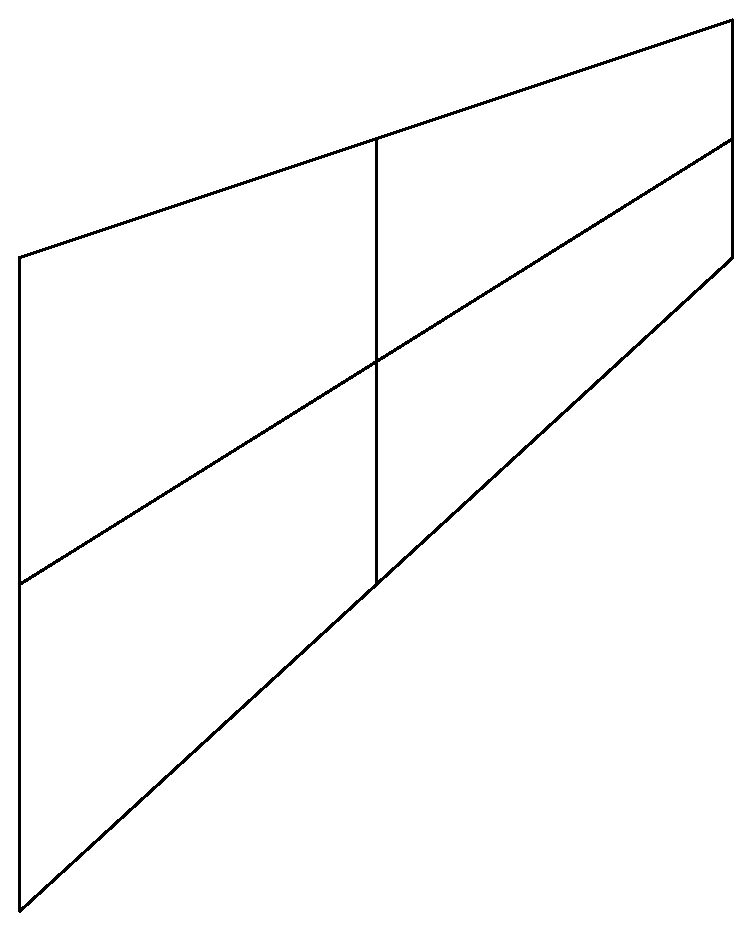
\includegraphics[width=20mm]{cook2}
\hfill
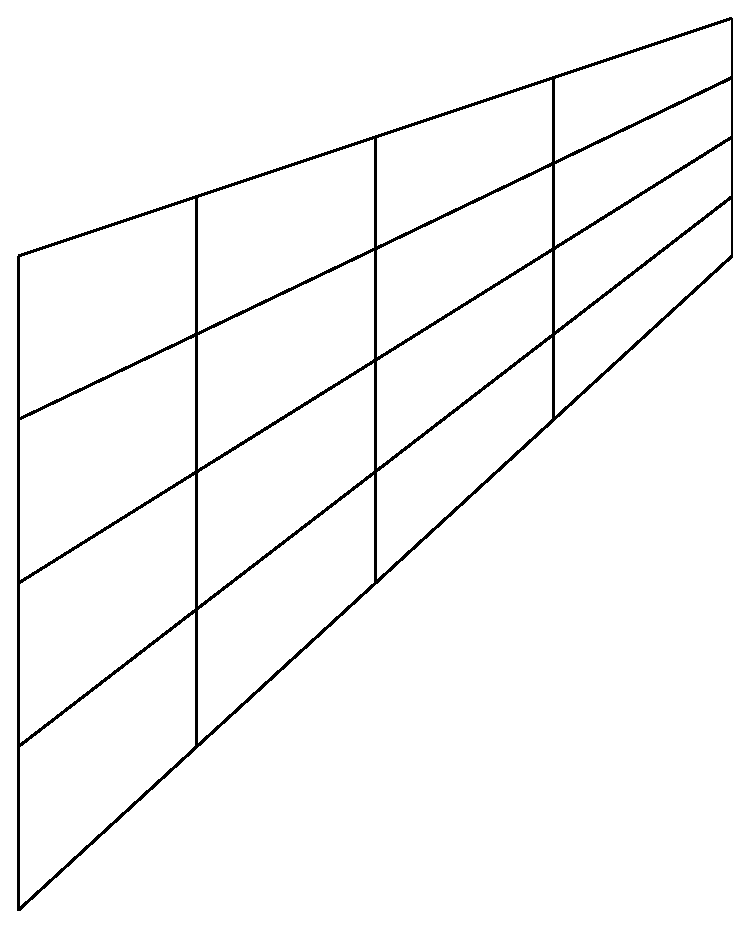
\includegraphics[width=20mm]{cook4}
\hfill
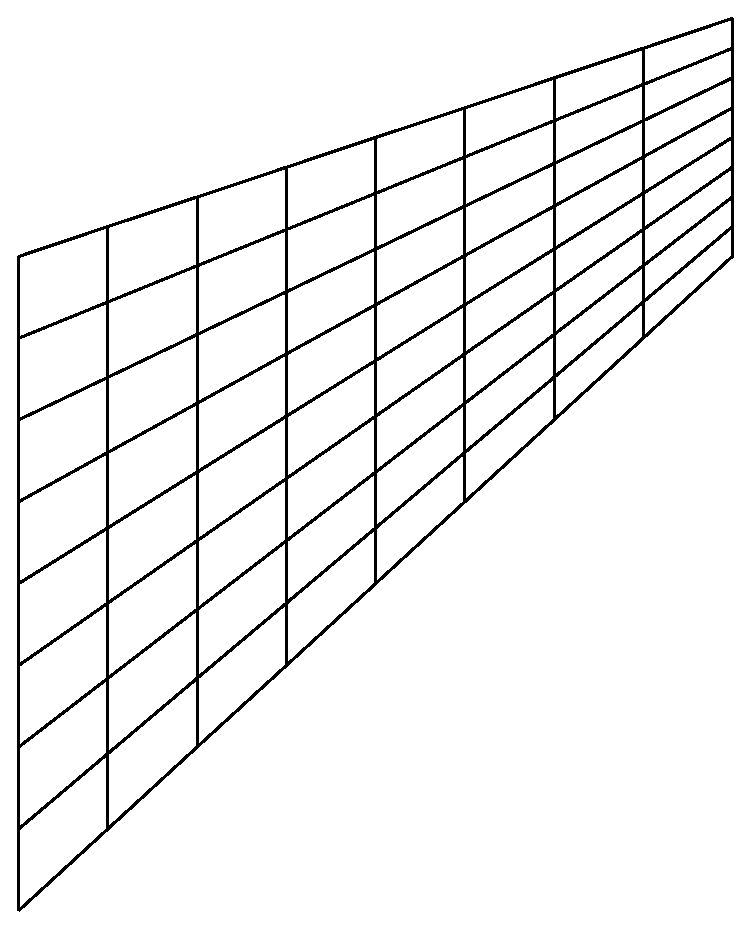
\includegraphics[width=20mm]{cook8}

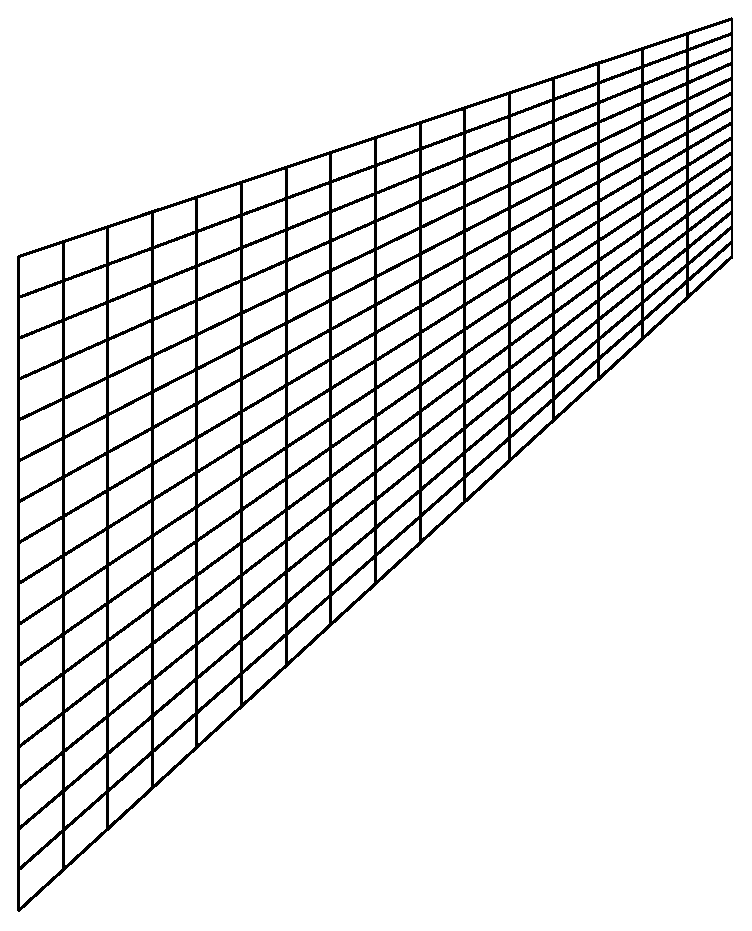
\includegraphics[width=20mm]{cook16}
\hfill
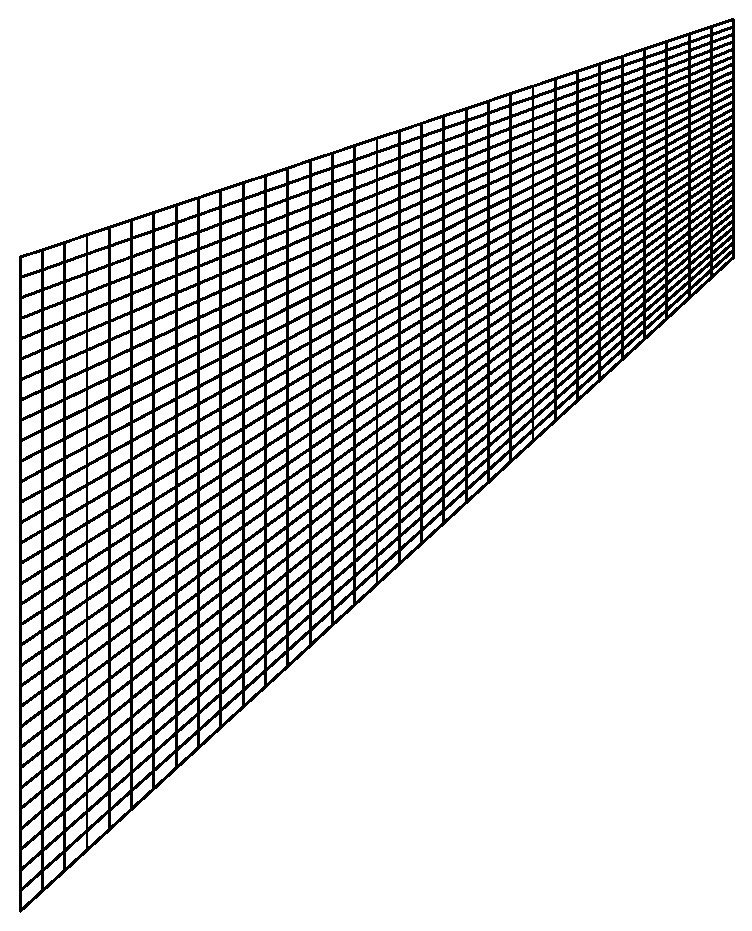
\includegraphics[width=20mm]{cook32}
\hfill
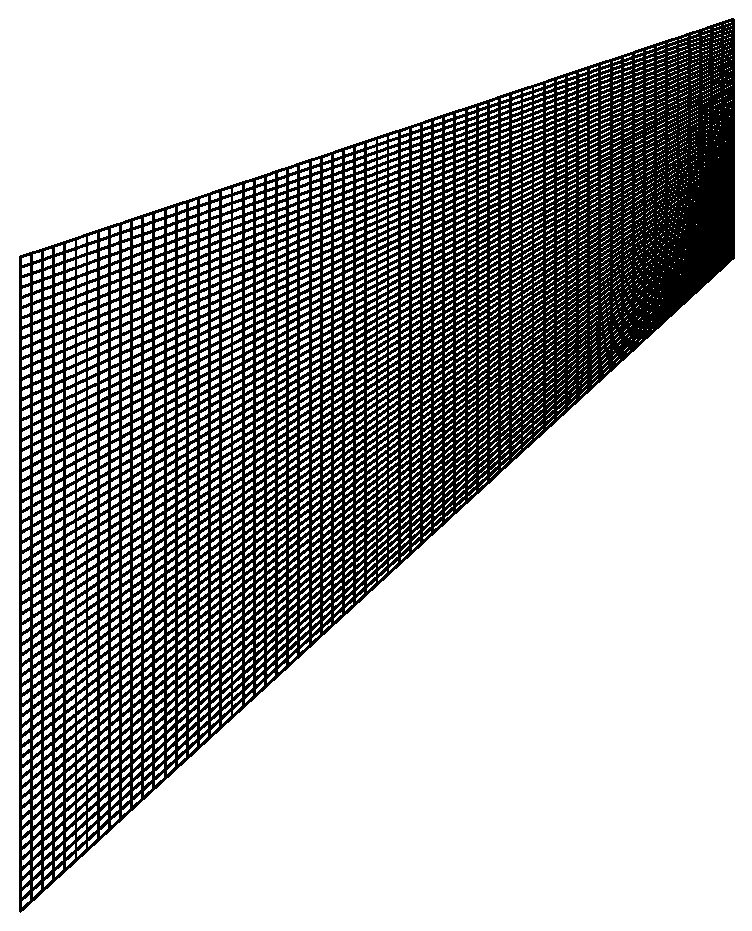
\includegraphics[width=20mm]{cook64}
\end{frame}
%%%%%%%%%%%%%%%%%%%%%%%%%%%%%%%%%%%%%%%%%%%%%%%%%%%%%%%%%%%%%%%%%%%%%%%%%%%%%%
\begin{frame}

\frametitle{Ejemplos. La membrana de Cook}
\begin{center}
\includegraphics[width=\textwidth]{cookcon}
\end{center}
\begin{align}
v &:\textrm{ Flecha} \nonumber \\
N &:\textrm{ Elementos por lado} \nonumber
\end{align}
\end{frame}
%%%%%%%%%%%%%%%%%%%%%%%%%%%%%%%%%%%%%%%%%%%%%%%%%%%%%%%%%%%%%%%%%%%%%%%%%%
\end{document}
